%%%%%%%%%%%%%%%%%%%%%%%%%%%%%%%%%%%%%%%%%%%%%%%%%%%%%%%%%%%%%%%%%%%%%%%%
%                                                                      %
%     File: Thesis_Appendix_A.tex                                      %
%     Tex Master: Thesis.tex                                           %
%                                                                      %
%     Author: Andre C. Marta                                           %
%     Last modified : 27 Feb 2024                                      %
%                                                                      %
%%%%%%%%%%%%%%%%%%%%%%%%%%%%%%%%%%%%%%%%%%%%%%%%%%%%%%%%%%%%%%%%%%%%%%%%

\chapter{Average Best-so-Far correction}
\label{Appendix:AvgBestSoFarCorrection}

Here are the revised plots illustrating the average best-so-far metric for the numerous heuristics tested throughout this study.

% For the 8-node graph:
\begin{figure*}[hb!]
    \centering
    \begin{subfigure}[t]{0.495\textwidth}
        \centering
        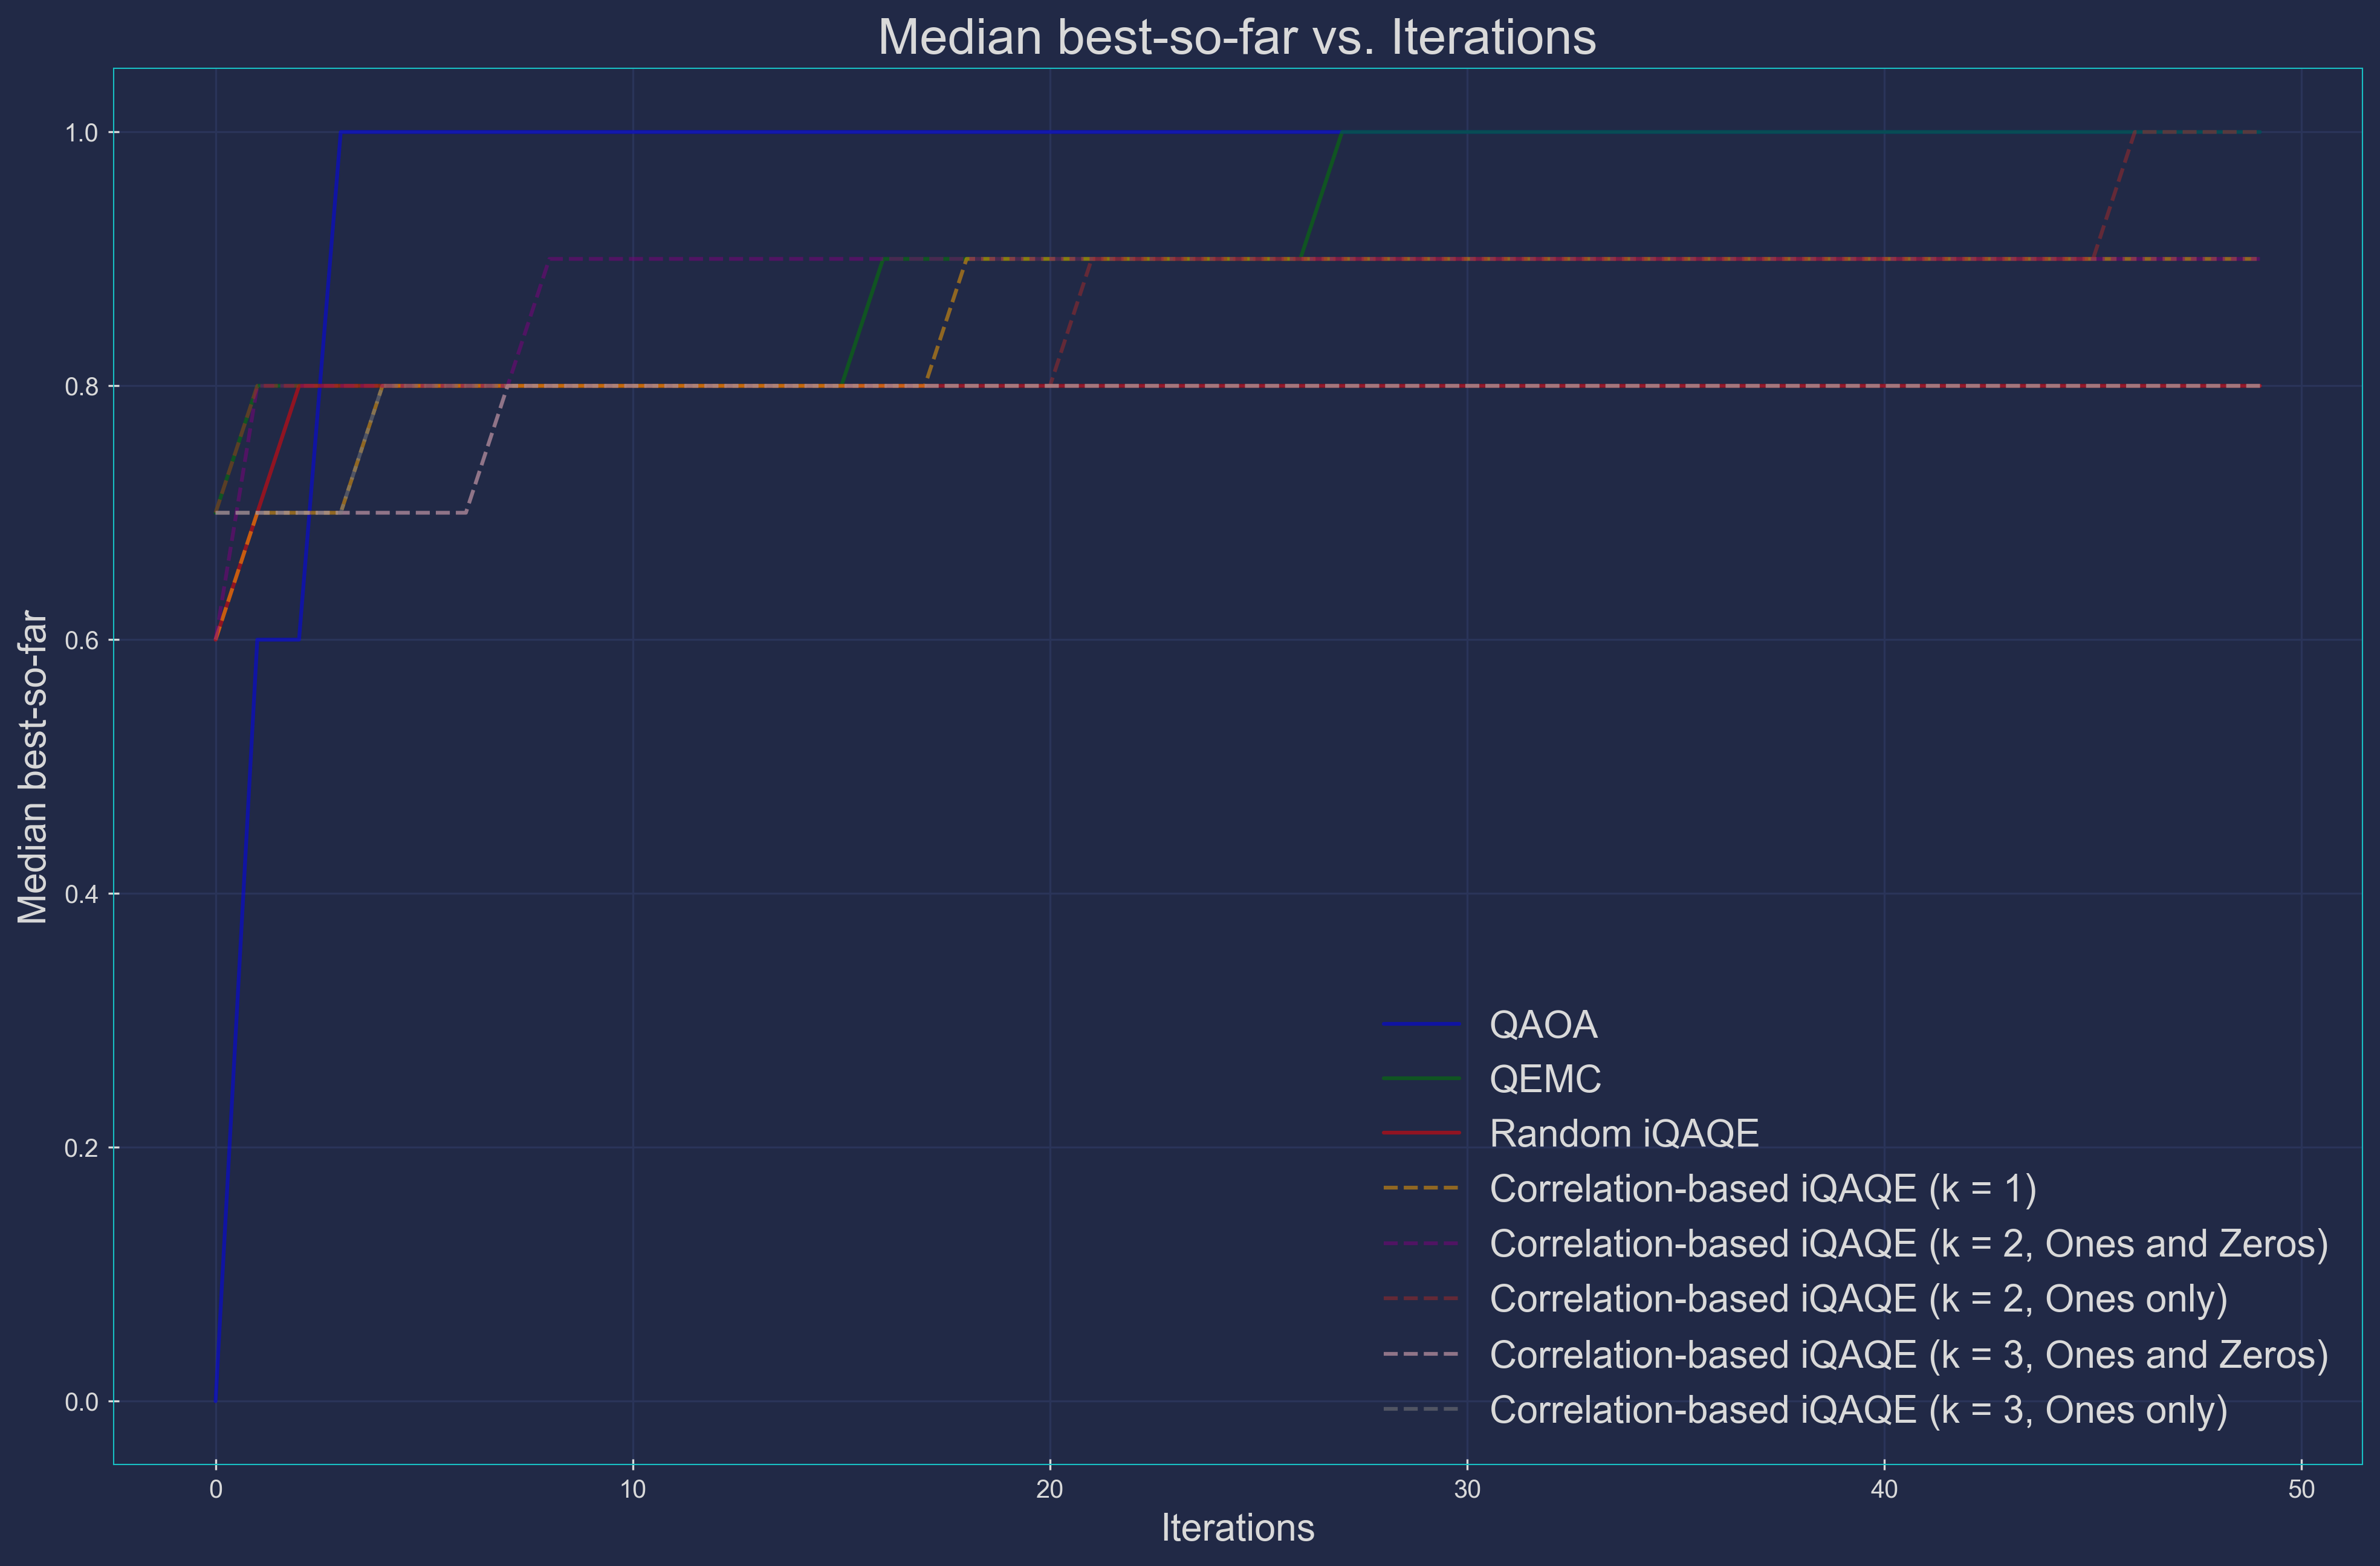
\includegraphics[width=1\textwidth]{Figures/Appendix_A/8-node/Basic+Correlation_iQAQE(8-node).png}
        \caption{Correlation-based schemes compared to \acrshort{qaoa}, \acrshort{qemc}, and a randomly chosen \acrshort{iqaqe} instance.}
        \label{fig:C_BSF_1_8-node}
    \end{subfigure}
    \hfill
    \begin{subfigure}[t]{0.495\textwidth}
        \centering
        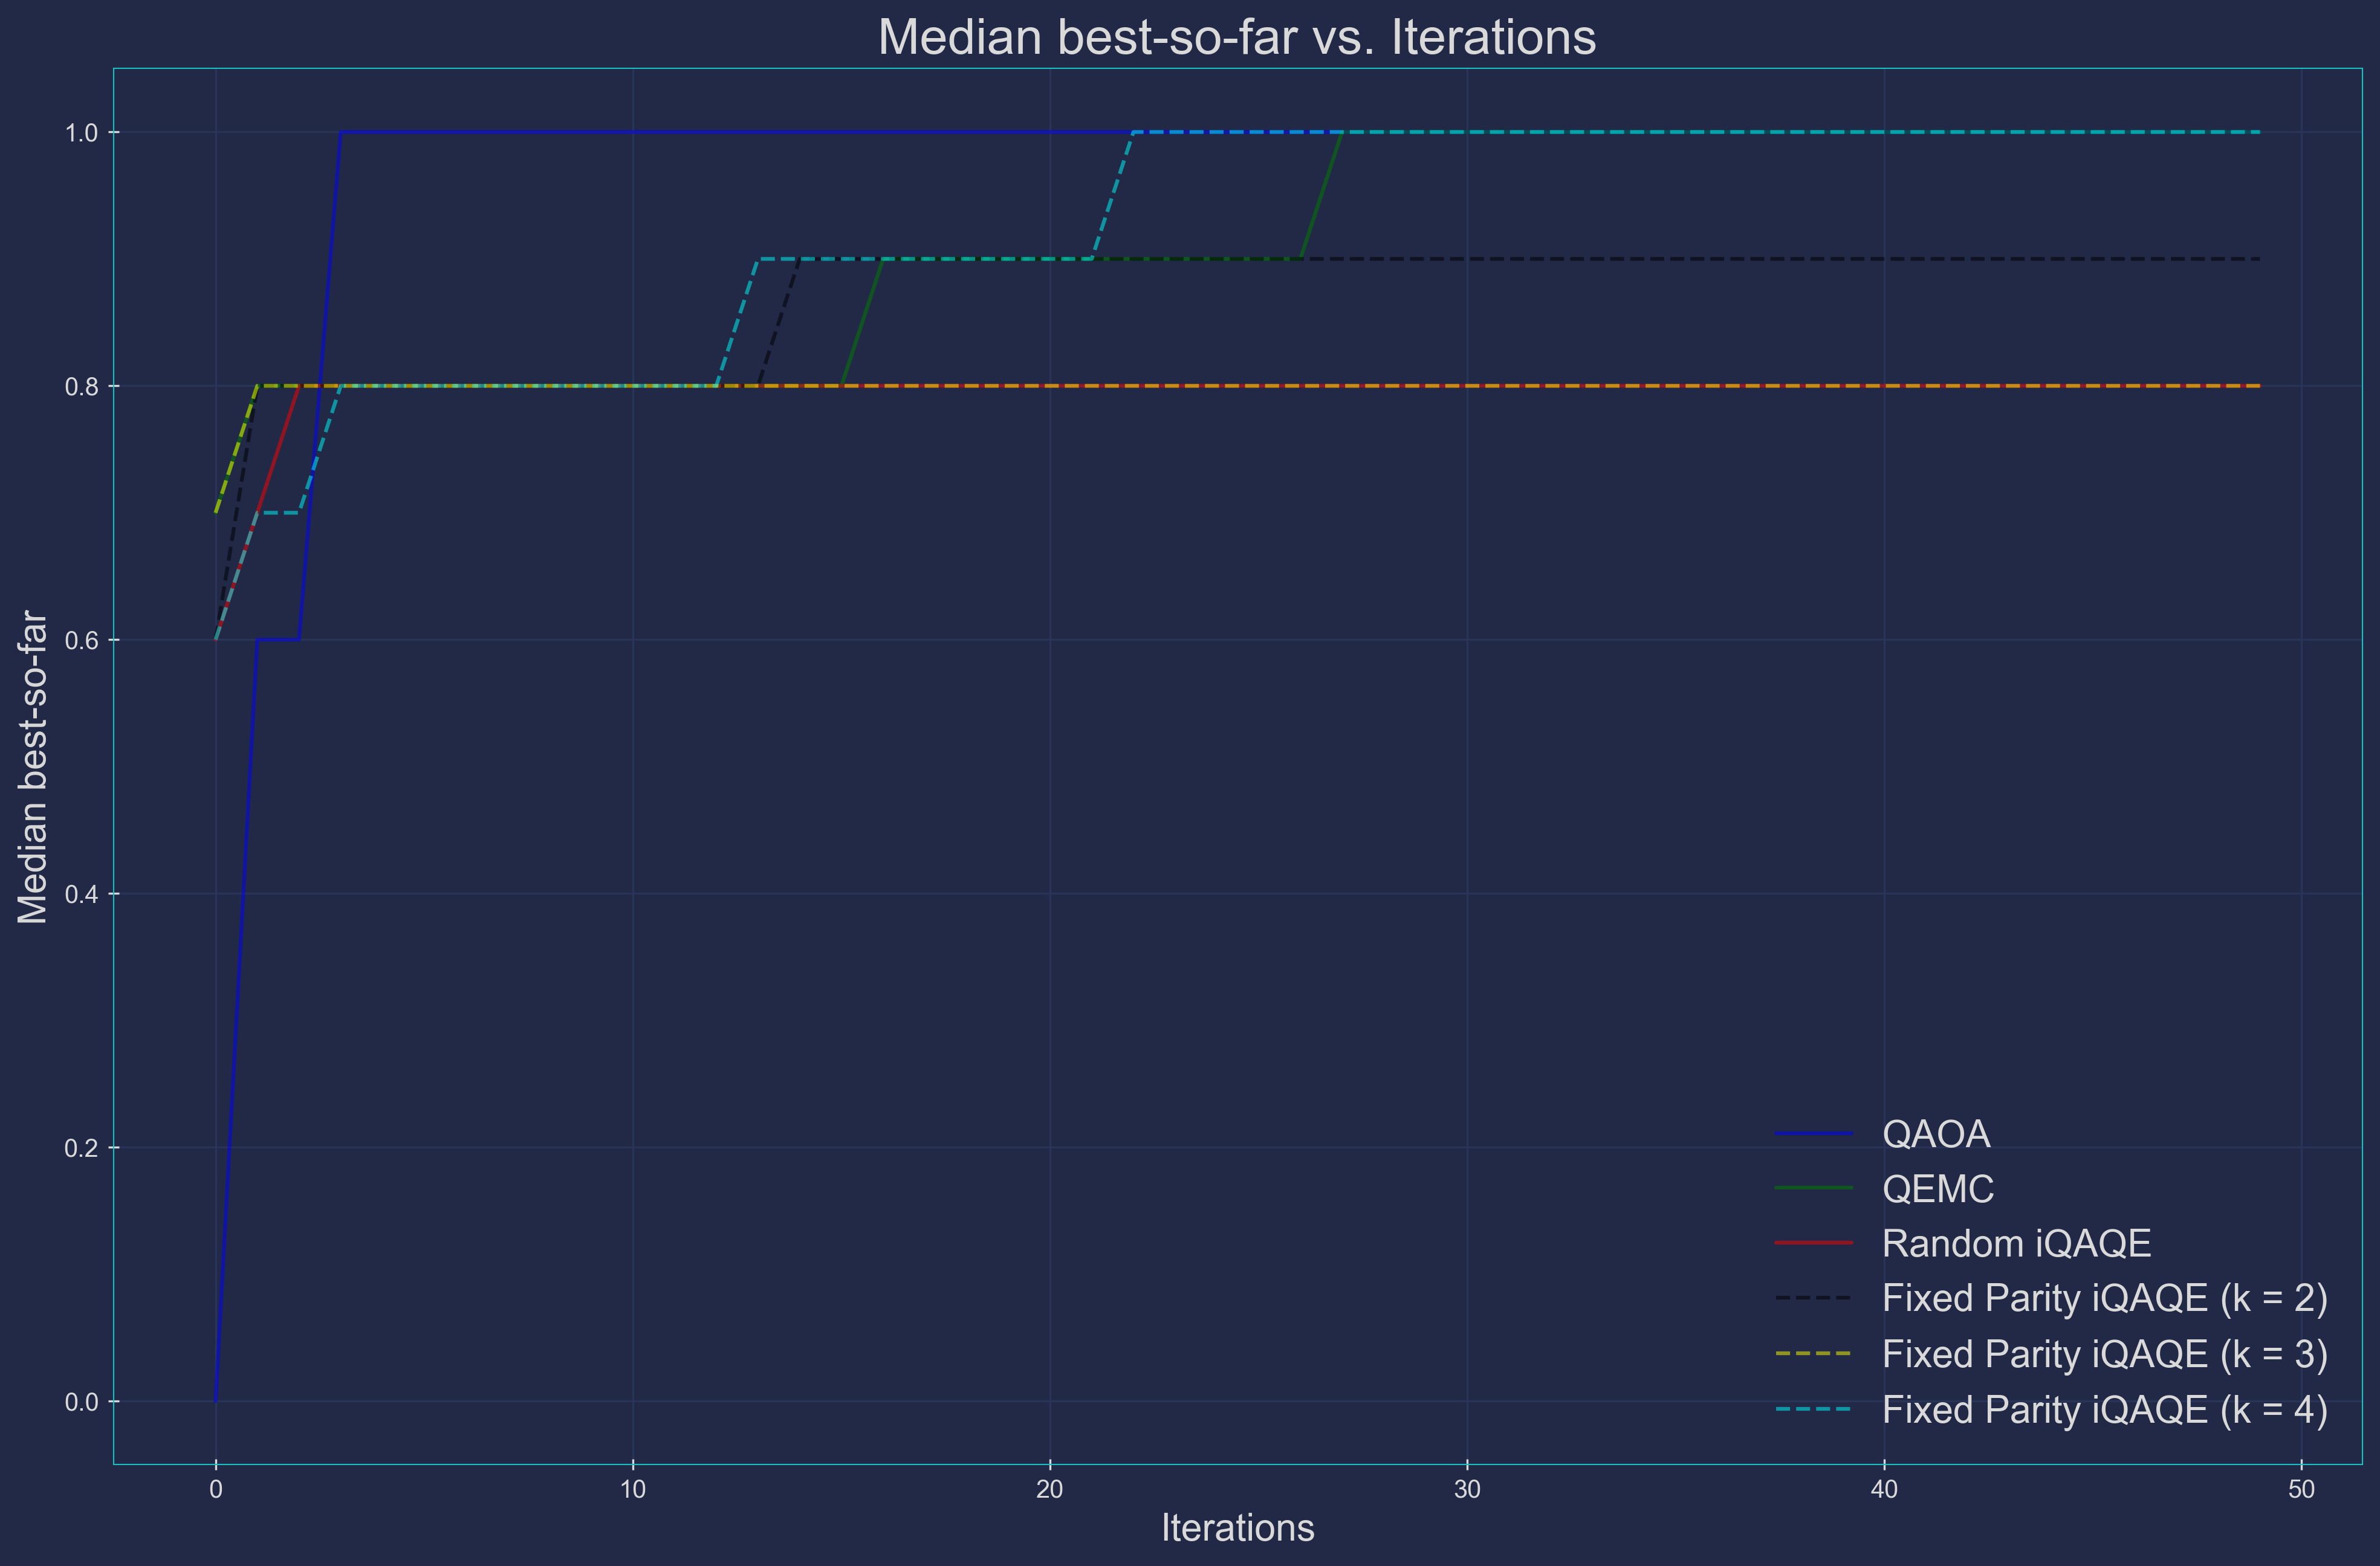
\includegraphics[width=1\textwidth]{Figures/Appendix_A/8-node/Basic+Fixed_Parity_iQAQE(8-node).png}
        \caption{Fixed-parity scheme compared to \acrshort{qaoa}, \acrshort{qemc}, and a randomly chosen \acrshort{iqaqe} instance.}
        \label{fig:C_BSF_2_8-node}
    \end{subfigure}
\end{figure*}

\begin{figure*}[ht!]
    \addtocounter{figure}{-1} % Added <<
    \centering
    \begin{subfigure}[t]{0.495\textwidth}
        \addtocounter{subfigure}{2} % Added <<
        \centering
        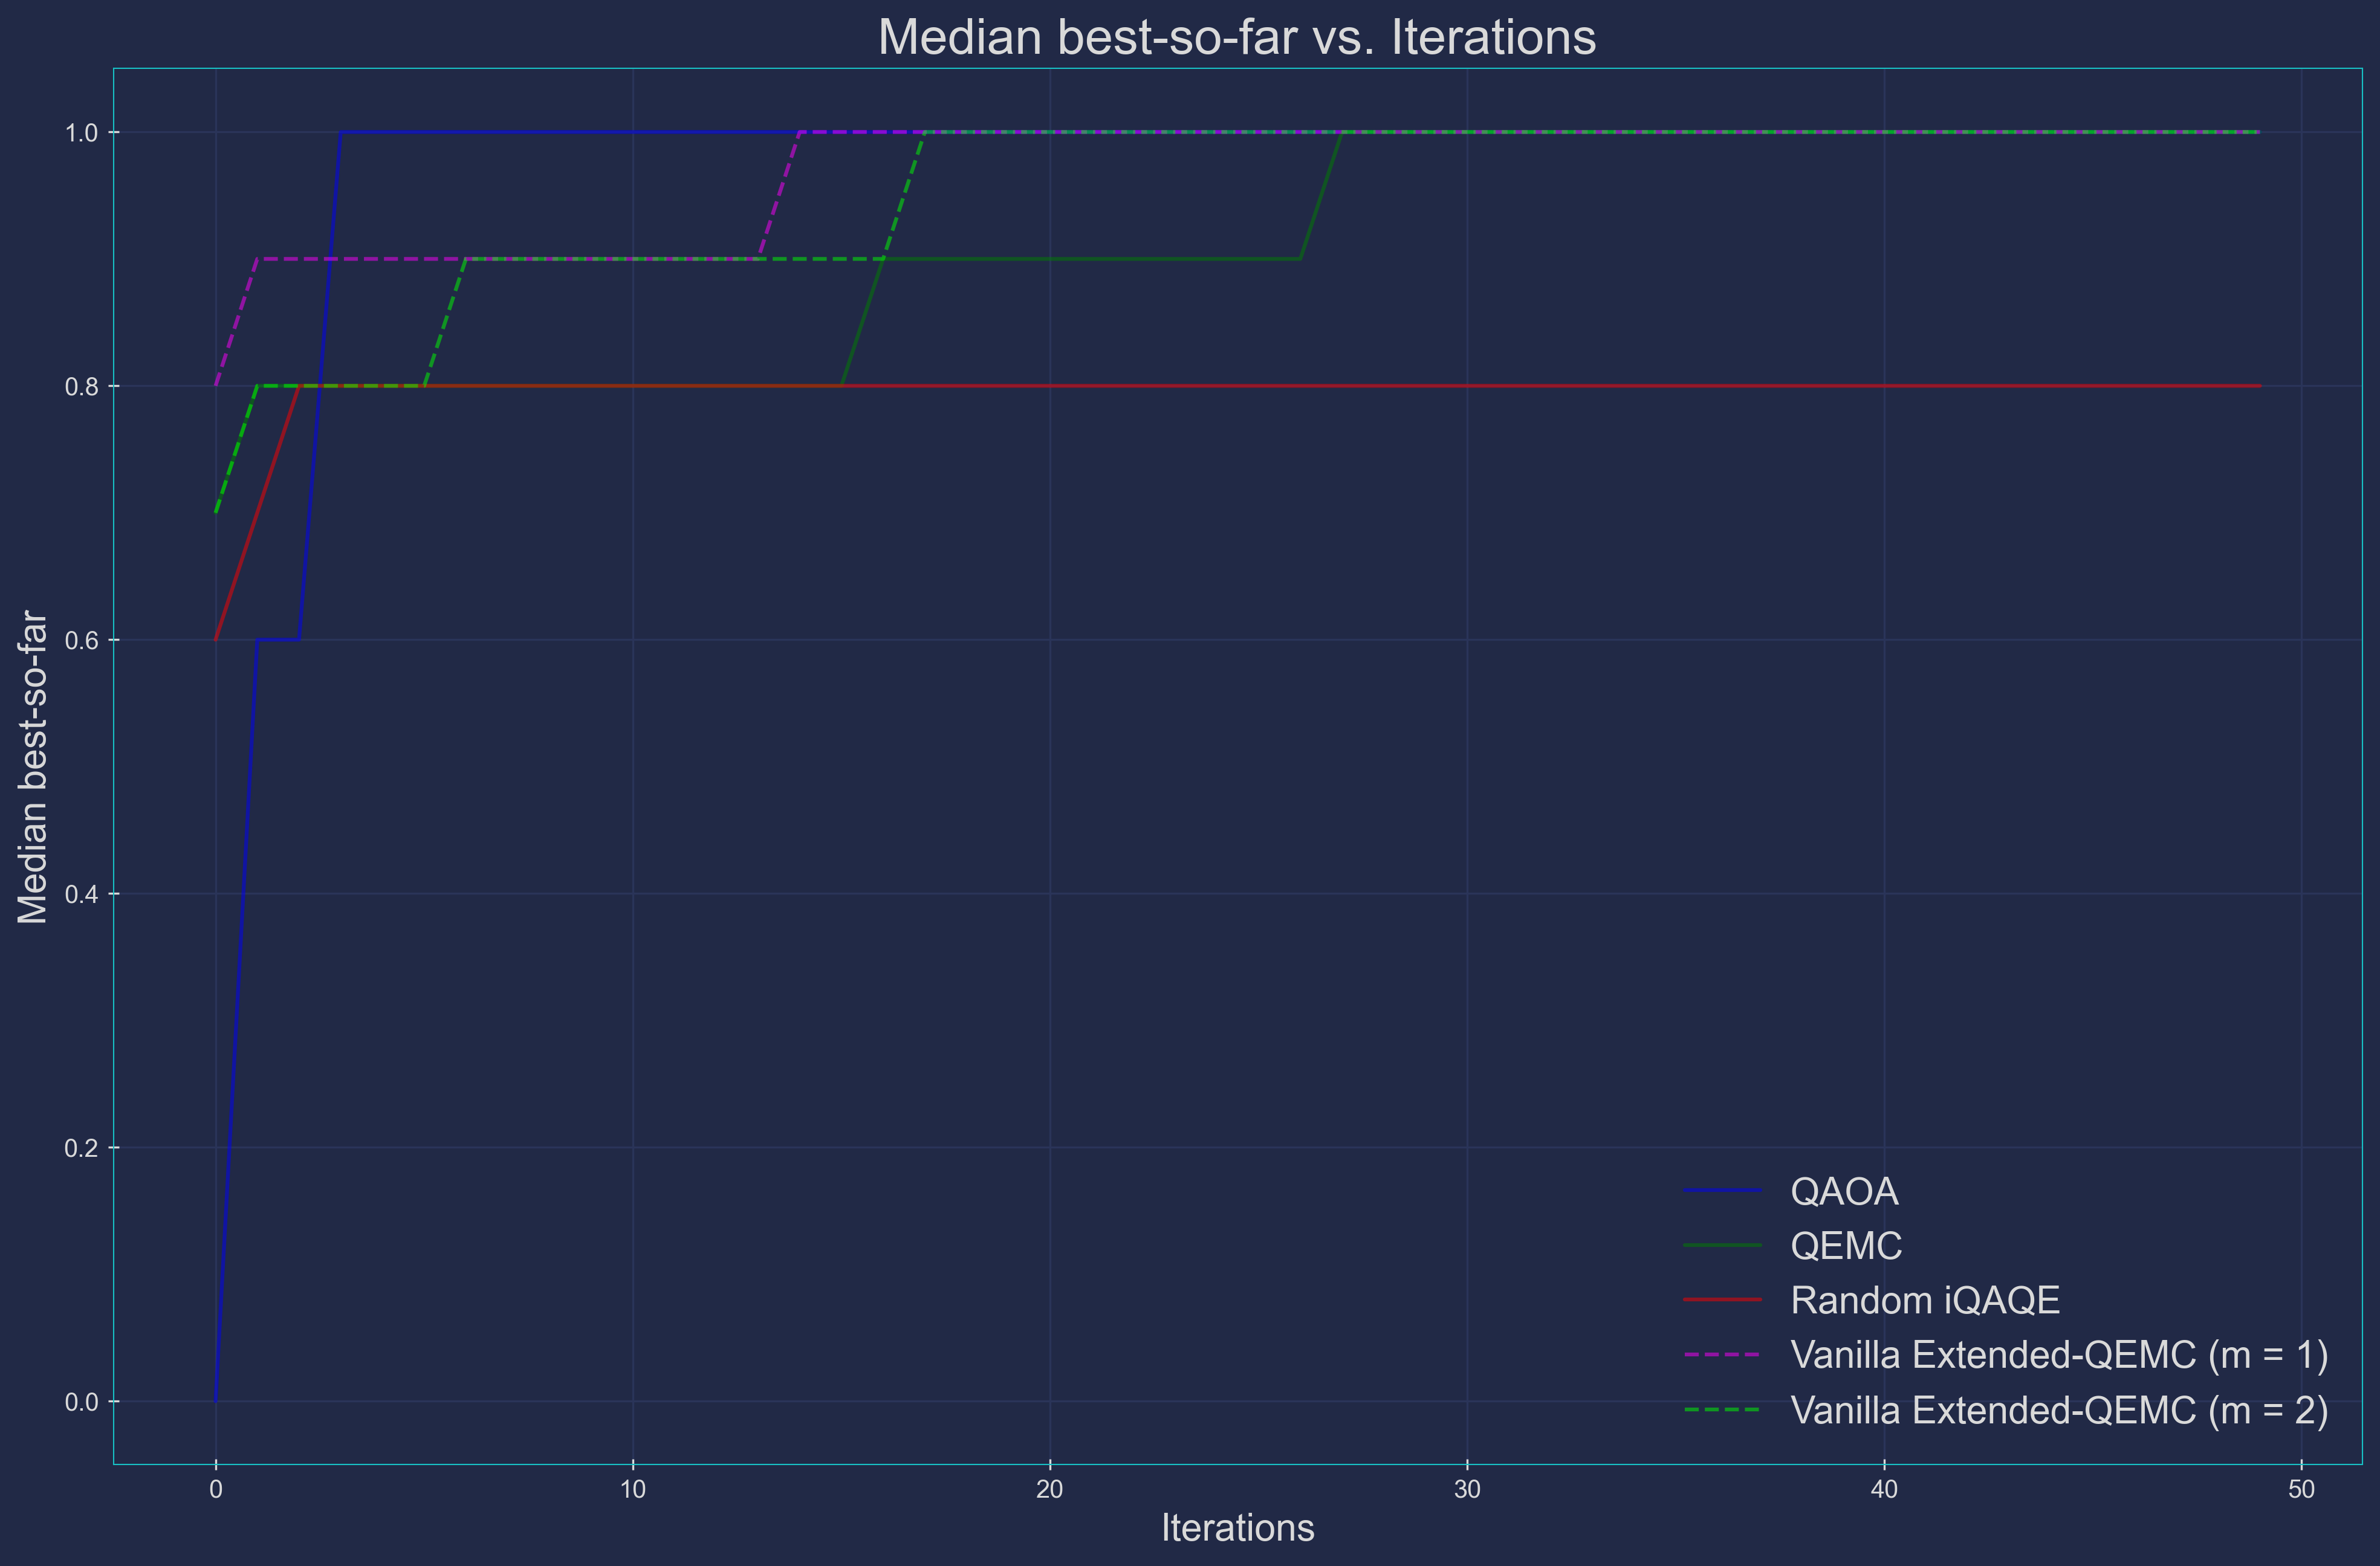
\includegraphics[width=1\textwidth]{Figures/Appendix_A/8-node/Basic+V_Extended_QEMC(8-node).png}
        \caption{Unmodified (Vanilla) Extended-QEMC scheme compared to \acrshort{qaoa}, \acrshort{qemc}, and a randomly chosen \acrshort{iqaqe} instance.}
        \label{fig:C_BSF_3_8-node}
    \end{subfigure}
    \hfill
    \begin{subfigure}[t]{0.495\textwidth}
        \centering
        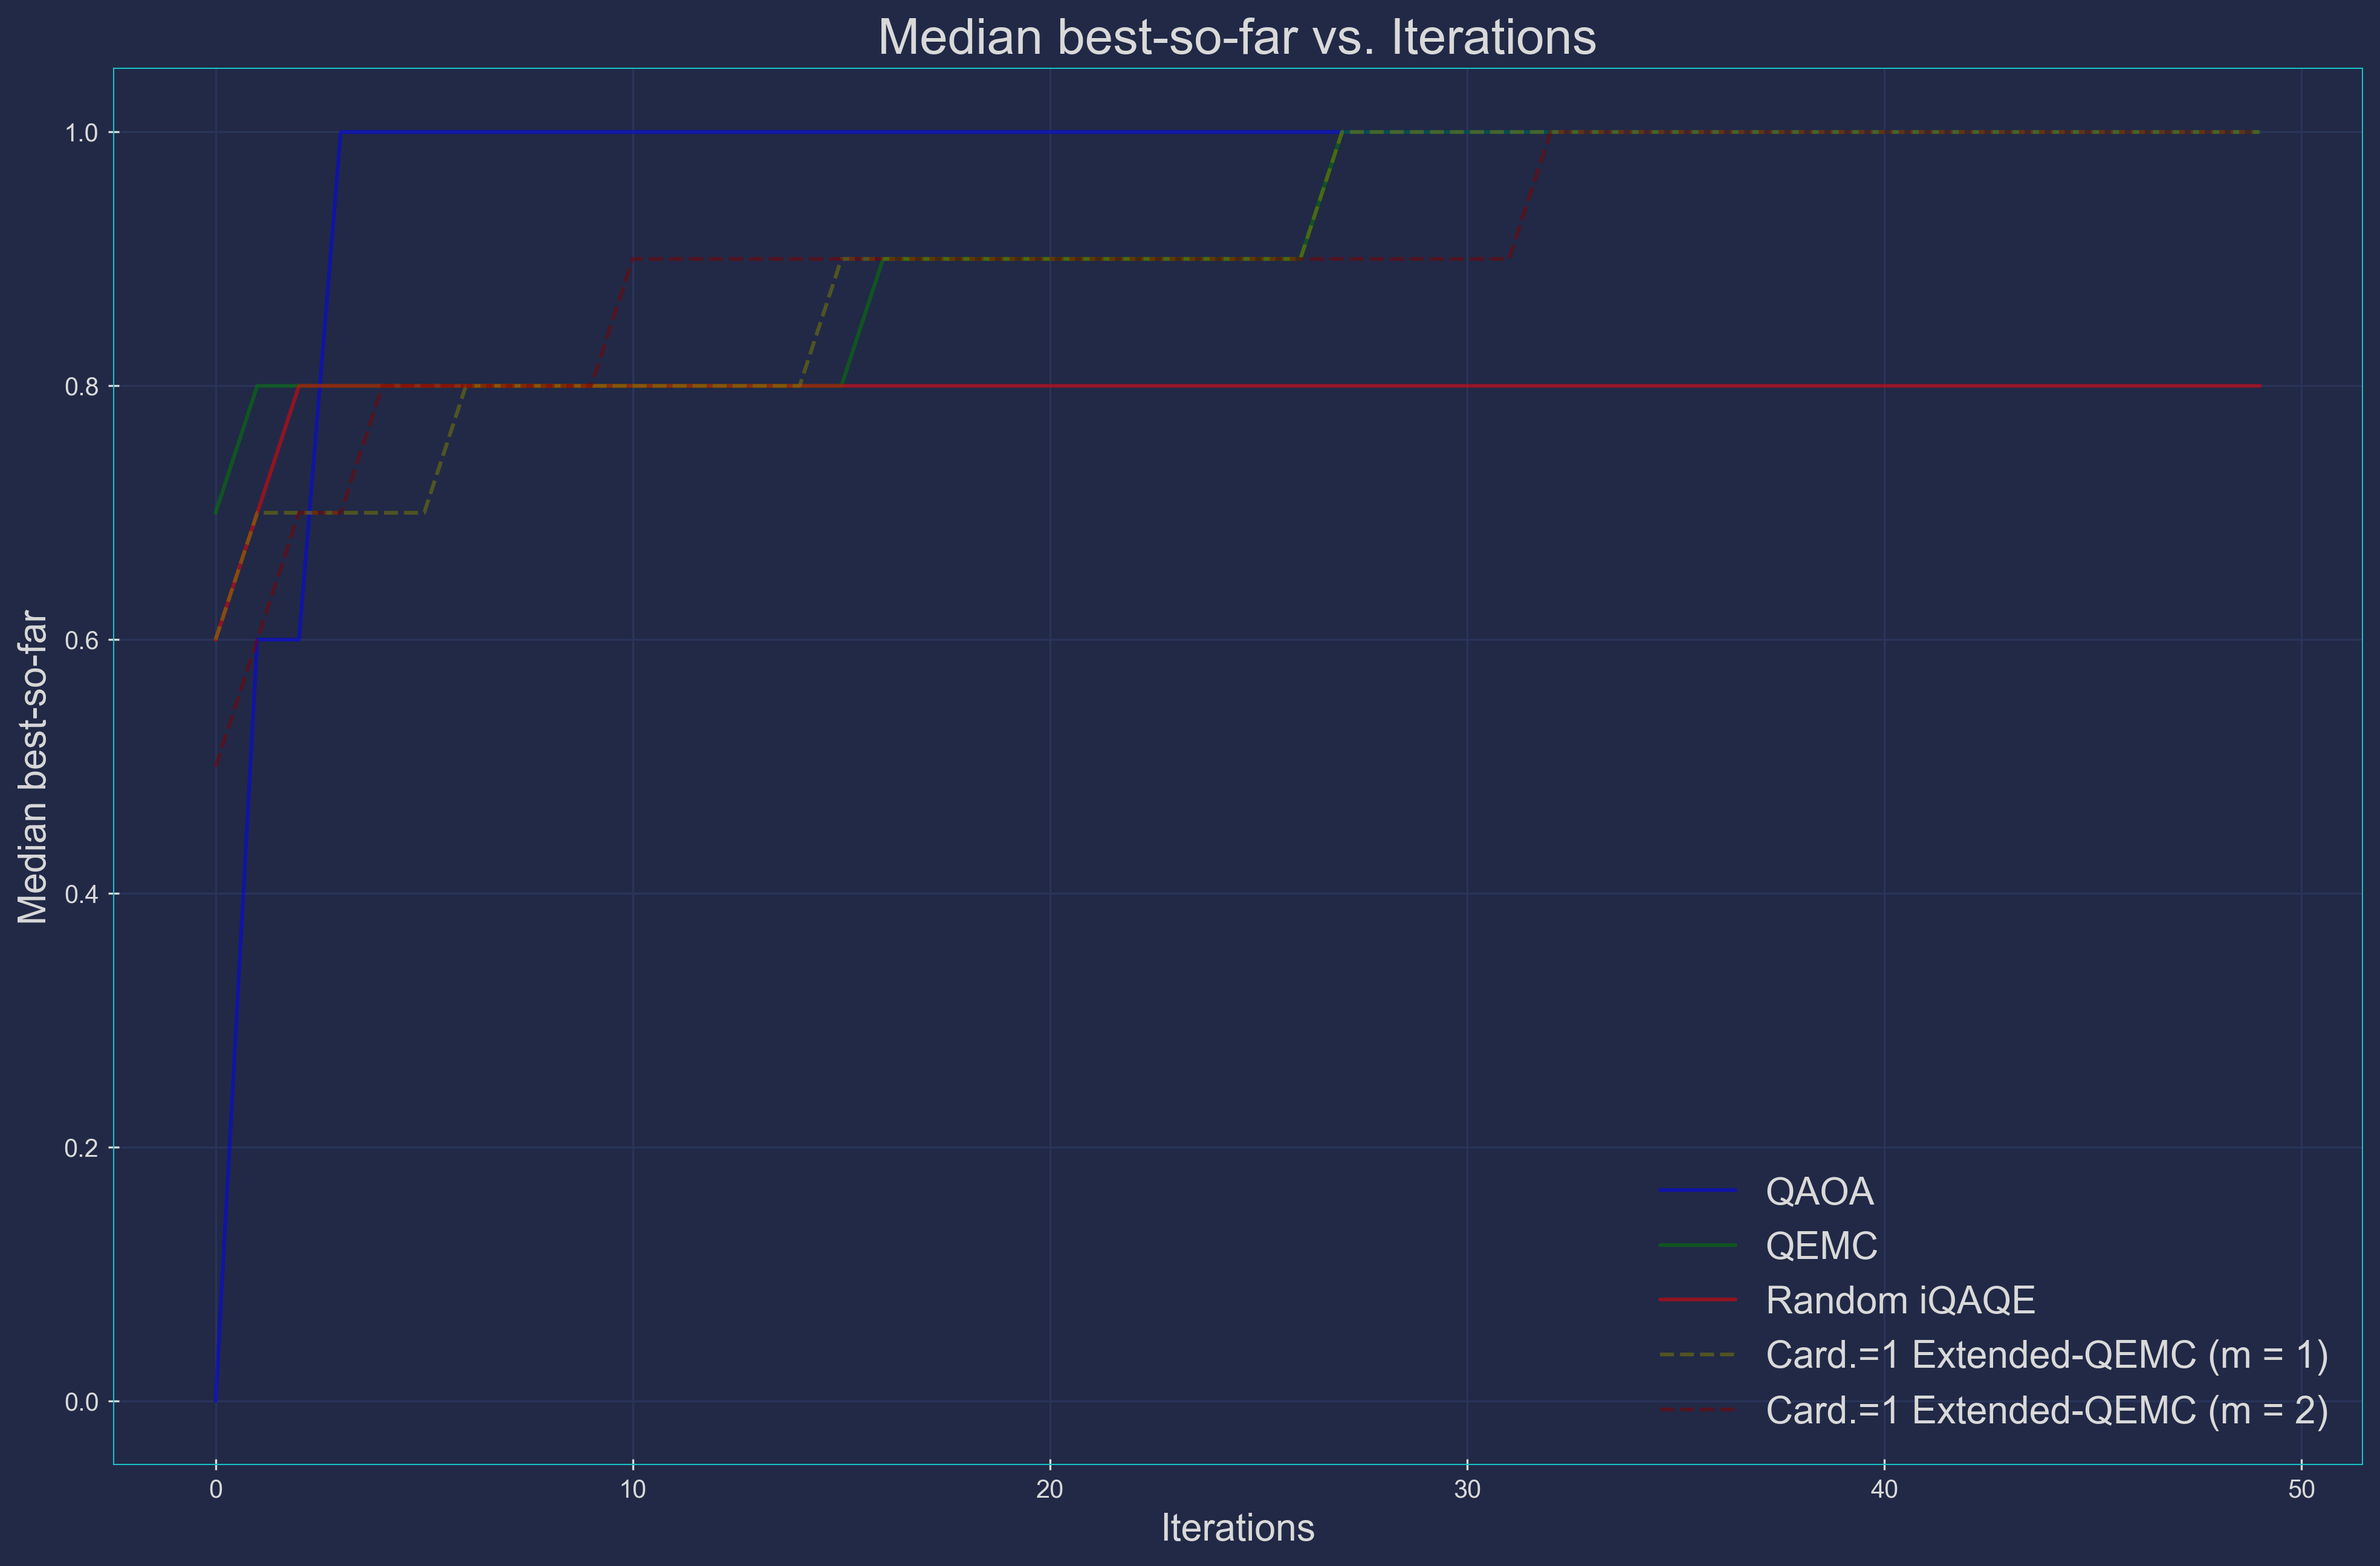
\includegraphics[width=1\textwidth]{Figures/Appendix_A/8-node/Basic+C1_Extended_QEMC(8-node).png}
        \caption{Cardinality $= 1$ Extended-QEMC scheme compared to \acrshort{qaoa}, \acrshort{qemc}, and a randomly chosen \acrshort{iqaqe} instance.}
        \label{fig:C_BSF_4_8-node}
    \end{subfigure}
\end{figure*}

\clearpage

\begin{figure*}[ht!]
	\addtocounter{figure}{-1} % Added <<
    \centering
	\begin{subfigure}[t]{1\textwidth}
		\addtocounter{subfigure}{2}
		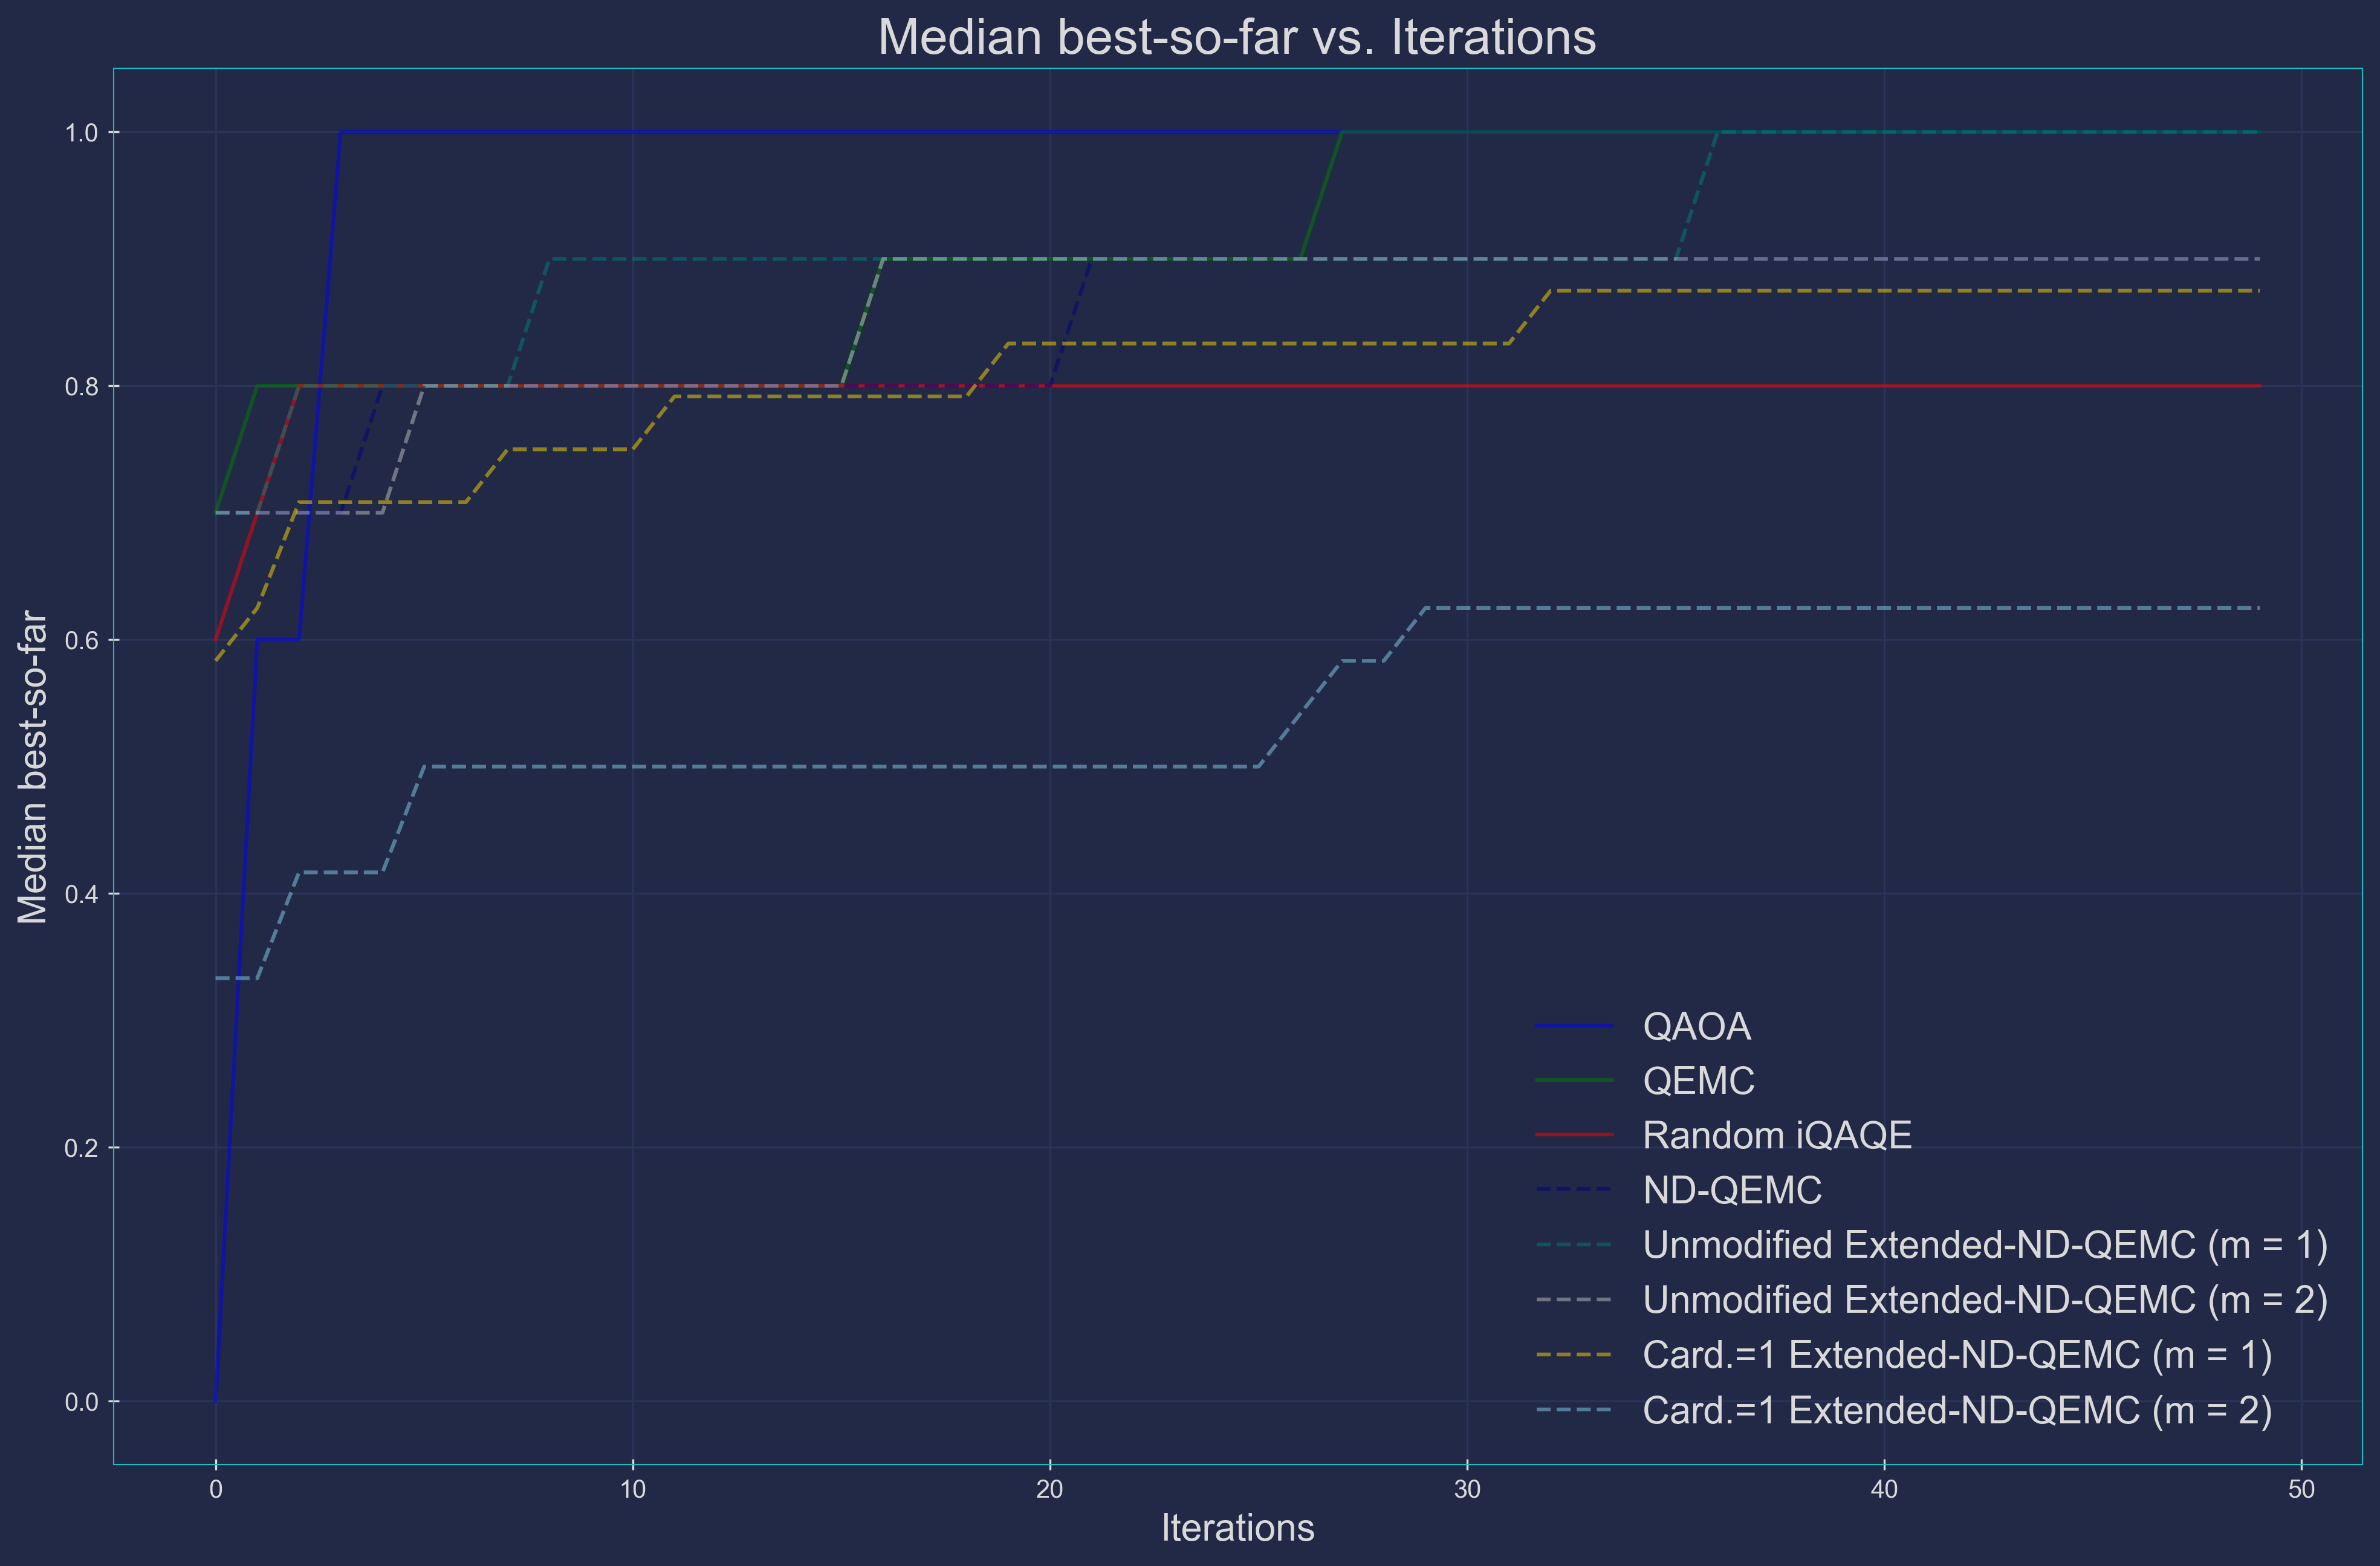
\includegraphics[width=1\textwidth]{Figures/Appendix_A/8-node/Basic+ND_QEMC_Variations(8-node).png}
		\caption{Non-deterministic CNOT-gate-using schemes compared to \acrshort{qaoa}, \acrshort{qemc}, and a randomly chosen \acrshort{iqaqe} instance.}
		\label{fig:C_BSF_5_8-node}
	\end{subfigure}
    \caption{Revised results using the corrected median best-so-far metric for the $8$-node graph.}
    \label{fig:Corrected_BSF_Results_8-node-graph}
\end{figure*}
